\documentclass[11pt,a4aper]{article}
\pdfoutput=1

\renewcommand{\baselinestretch}{1}
\usepackage[UKenglish]{isodate}
\cleanlookdateon

%%%%% Fonts, symbols, colours, microtypography
\usepackage{amsfonts,amsmath,amssymb,amsthm,mathtools,microtype} % Symbols & microtypography
\usepackage[dvipsnames]{xcolor} % Colours with names -- see https://www.overleaf.com/learn/latex/Using_colours_in_LaTeX for list
\usepackage[noBBpl]{mathpazo} % Palatino, but not for mathbb

%%%%% Figures, tables, lists
\usepackage[labelsep=period,labelfont=bf,justification=centering]{caption}
\usepackage{float,graphicx,subcaption}
\usepackage{enumitem}
\setlist[itemize]{topsep=0ex,itemsep=0ex,parsep=0.4ex}
\setlist[enumerate]{topsep=0ex,itemsep=0ex,parsep=0.4ex}

\usepackage{parskip,fullpage}
\usepackage{thm-restate}
\usepackage[textsize=scriptsize]{todonotes}
\setlength{\marginparwidth}{2cm}%to have larger todonotes
\usepackage{comment}

\usepackage{array}


%%%%% Hyperlinking
\usepackage[hyphens]{url} % Urls together with line breaking them
\usepackage[linktoc=all,hidelinks,colorlinks,unicode=true]{hyperref} % Must be loaded after url
\usepackage[capitalise,compress,nameinlink,noabbrev]{cleveref} % Must be loaded after hyperref
\hypersetup{linkcolor={blue!70!black},citecolor={black},urlcolor={blue!70!black}}
\usepackage{hyperref}

\usepackage{tikz}

\newtheorem{theorem}{Theorem}
\newtheorem{lemma}{Lemma}[section]
\newtheorem{claim}[lemma]{Claim}
\newtheorem*{claim*}{Claim}
\newtheorem{conjecture}{Conjecture}
\newtheorem{corollary}[lemma]{Corollary}
\newtheorem{question}[lemma]{Question}
\theoremstyle{definition}
\newtheorem{remark}[lemma]{Remark}
\newtheorem{problem}[lemma]{Problem}

\makeatletter
\def\namedlabel#1#2{\begingroup
   \def\@currentlabel{#2}%
   \label{#1}\endgroup
}
\makeatother

\newenvironment{poc}{\begin{proof}[Proof of
    Claim]\renewcommand*{\qedsymbol}{$\blacksquare$}}{\end{proof}}

\crefname{subsection}{Subsection}{Subsections}

%%%%% Renew commands

\renewcommand{\ge}{\geqslant}
\renewcommand{\le}{\leqslant}
\renewcommand{\geq}{\geqslant}
\renewcommand{\leq}{\leqslant}
% \renewcommand{\eps}{\varepsilon}
\renewcommand{\emptyset}{\varnothing}

%%%%% mathbold and mathcal
\newcommand*{\eps}{\varepsilon}
\newcommand*{\bE}{\mathbb{E}}
\newcommand*{\bN}{\mathbb{N}}
\newcommand*{\bP}{\mathbb{P}}
\newcommand*{\bR}{\mathbb{R}}
\newcommand*{\bZ}{\mathbb{Z}}
\newcommand*{\cF}{\mathcal{F}}
\newcommand*{\cO}{\mathcal{O}}
\newcommand*{\cE}{\mathcal{E}}
\newcommand*{\cI}{\mathcal{I}}
\newcommand*{\cJ}{\mathcal{J}}
\newcommand*{\cR}{\mathcal{R}}
\newcommand*{\cC}{\mathcal{C}}
\newcommand*{\cX}{\mathcal{X}}
\newcommand*{\cG}{\mathcal{G}}
\newcommand*{\cY}{\mathcal{Y}}
\newcommand*{\cB}{\mathcal{B}}
\newcommand*{\cS}{\mathcal{S}}
\newcommand*{\cD}{\mathcal{D}}
\newcommand*{\cM}{\mathcal{M}}
\newcommand*{\cP}{\mathcal{P}}
\newcommand*{\cQ}{\mathcal{Q}}
\newcommand*{\cA}{\mathcal{A}}
\newcommand*{\cU}{\mathcal{U}}
\DeclareMathOperator{\sq}{\square}

\DeclarePairedDelimiter{\set}{\{}{\}}
\DeclarePairedDelimiter{\abs}{\lvert}{\rvert}
\DeclarePairedDelimiter{\floor}{\lfloor}{\rfloor}
\DeclarePairedDelimiter{\ceil}{\lceil}{\rceil}

% Colors
\newcommand{\colora}{Goldenrod}
\newcommand{\colorb}{SkyBlue}
\newcommand{\colorc}{Sepia}
\newcommand{\colord}{orange}
\newcommand{\colore}{MidnightBlue}
\newcommand{\colorf}{white}
\newcommand{\colorg}{black}

\newcommand{\cola}{\coloredbullet{\colora}}
\newcommand{\colb}{\coloredbullet{\colorb}}
\newcommand{\colc}{\coloredbullet{\colorc}}
\newcommand{\cold}{\coloredbullet{\colord}}
\newcommand{\cole}{\coloredbullet{\colore}}
\newcommand{\colf}{\coloredbullet{\colorf}}
\newcommand{\colg}{\coloredbullet{\colorg}}

  
%%% Comments
\newcommand{\bartosz}[1]{{\color{blue} BW: #1}}
\newcommand{\clement}[1]{{\color{orange} CL: #1}}
\newcommand{\nicolas}[1]{{\color{purple} UG: #1}}
\newcommand{\ugo}[1]{{\color{red} NT: #1}}

\title{Shift graph recognition is NP-complete}

\date{\today}

\author{
Bartosz Walczak\footnotemark[1] \and 
Cl\'ement Legrand-Duchesne\footnotemark[1]\and
Ugo Giocanti\footnotemark[1] \and
Nicolas Trotignon\footnotemark[4]
}

\begin{document}
\maketitle

\renewcommand{\thefootnote}{\fnsymbol{footnote}} % Make affiliation marks symbols

\footnotetext[1]{Theoretical Computer Science Department, Faculty of Mathematics and Computer Science, Jagiellonian University, Kraków, Poland.}
\footnotetext[2]{}

\renewcommand{\thefootnote}{\arabic{footnote}} % Return to normal footnote symbols

\begin{abstract}
\end{abstract}


Given a digraph $D$, the \emph{line digraph} $L(D)$ of $D$ is the digraph whose
vertices are the arcs of $D$ and in which there is an arc from $a$ to $b$ if the
head of $a$ is the tail of $b$ in $D$. The \emph{$k$-iterated line digraph} $L^k(D)$
of $D$ is then defined recursively by $L^k(D) = L(L^{k-1}(D))$ and $L^0(D) = D$.
Equivalently, the vertices of $L^k(D)$ are the directed path on $k+1$ vertices
in $D$ and $L^k(D)$ contains an arc from $a$ to $b$ if the corresponding
directed path overlap on the $k$ last vertices of $a$ and the $k$ first vertices
of $b$, namely $a = (v_0, \dots v_k)$ and $b=(v_1, \dots v_{k+1})$ with
$(v_i,v_{i+1}) \in A(D)$ for all $i$. The \emph{support} of a digraph $D$ is the
non-directed graph $G$ obtained by removing the orientations of the arcs of $D$,
that is $V(G) = V(D)$ and $E(G) = \{\{x,y\} \colon (x,y) \in A(D)\}$. 

The shift graph $G_{n,k}$ is the graph whose vertices are ordered $k$-tuples
$(a_1, \dots a_k)$ of $[n]$ such that $1 \le a_1 < a_2 < \dots < a_k \le n$, in
which two vertices $a = (a_1, \dots a_k)$ and $b = (b_1, \dots b_k)$ are
adjacent if $b_i = a_{i+1}$ for all $i \in [k-1]$ (or $a_i = b_{i+1}$ for all
$i \in [k-1]$). From this definition, it is straightforward to check that
$G_{n,k}$ is the support of the $(k-1)$-iterated line digraph of the transitive
tournament on $n$ vertices. The graph $G_{n,k}$ has odd-girth $2k+1$, in
particular shift graphs are triangle-free.

The class of $k$-shift graphs (or simply shift graphs for $k=2$) is the
hereditary closure of the graphs $\{G_{n,k} : n \ge 1\}$, that is, all induced
subgraph of some $G_{n,k}$. Note that this definition is equivalent to saying
that $k$-shift graphs are the supports of the $(k-1)$-iterated line digraphs of
all directed acyclic graphs.

The following result of Beineke shows that line digraphs of digraphs can be
recognised in polynomial time.
\begin{lemma}[Beineke~\cite{beineke1968Derived}]
  A digraph $D$ is the line digraph of a digraph if and only if the two
  following conditions are satisfied:
  \begin{enumerate}
  \item If $D$ contains three arcs $a$, $b$ and $c$ such that $a$ and $b$ have
    the same tail, and $b$ and $c$ have the same head, then $D$ also contains an
    arc from the tail of $c$ to the head of $a$.
  \item $D$ does not contain four arcs $a$, $b$, $c$ and $d$ such that the tails
    of $a$ and $c$ are identical, the heads of $d$ and $b$ are identical, and
    the head of $a$ (resp. $c$) is the tail of $b$ (resp. $d$).  
  \end{enumerate}
\end{lemma}

However, Chv\'atal and Ebenegger showed that recognising their support is
NP-complete~\cite{chvatal1990Note}.



\section{Recognizing supports of line digraphs}
\clement{With Ugo, we noticed a mistake in our proof for high girth. Here is a
  sktch of proof for girth 4. We simplified the clause gadget to a path with
  four pending edges.}
\begin{theorem}
  Recognizing the support of a shift graph is an NP-complete problem.
\end{theorem}
\begin{proof}
  We reduce the ``not all equal'' 3-SAT problem to shift graph
  recognition.

  Let $\phi$ be a formula in conjonctive normal form, with three litterals per
  clause.

  Let $H$ be the four sun, that is the graph on eight vertices composed of a
  four-cycle and a pending edge attached to each of the vertices of the cycle.
  Let $m$ be the number of clauses. For each variable $x$, consider the
  gadget composed of a path on $8m-1$ vertices $u_x^0, \dots u_x^{8m-2}$ in which
  we connect each $u_x^{2i}$ to a vertex $v_x^{2i}$ itself adjacent to $w_x^{2i}$
  and to a copy of $H$ via one of the
  vertices of degree three (see \cref{fig:variable_gadget}).

  \begin{figure}[h!]
    \centering
    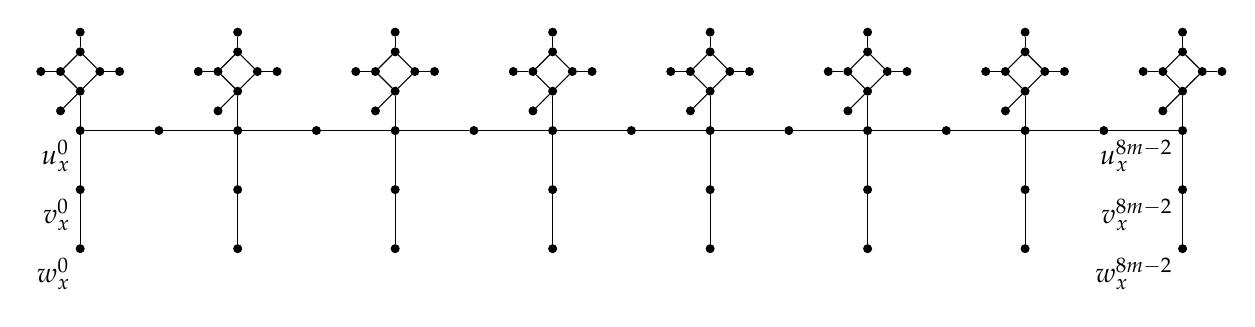
\begin{tikzpicture}[scale = 1]
      \foreach \i in {0,...,7}{
        \begin{scope}[shift={(2*\i,0)}]
          \node[draw,circle,fill=black,inner sep=1pt] (a\i) at (0,0) {};
          
          \node[draw,circle,fill=black,inner sep=1pt] (e\i1) at (0,-.75) {};
          \node[draw,circle,fill=black,inner sep=1pt] (e\i2) at (0,-1.5) {};

          \node[draw,circle,fill=black,inner sep=1pt] (H\i11) at (0,.5) {};
          \node[draw,circle,fill=black,inner sep=1pt] (H\i12) at (-.25,.25) {};
          \node[draw,circle,fill=black,inner sep=1pt] (H\i21) at (.25,.75) {};
          \node[draw,circle,fill=black,inner sep=1pt] (H\i22) at (.5,.75) {};
          \node[draw,circle,fill=black,inner sep=1pt] (H\i31) at (0,1) {};
          \node[draw,circle,fill=black,inner sep=1pt] (H\i32) at (0,1.25) {};
          \node[draw,circle,fill=black,inner sep=1pt] (H\i41) at (-.25,.75) {};
          \node[draw,circle,fill=black,inner sep=1pt] (H\i42) at (-.5,.75) {};
          \draw (H\i11) -- (H\i21) -- (H\i31) -- (H\i41) -- (H\i11);
          \draw (H\i11) -- (a\i) -- (e\i1) -- (e\i2) ;
          \foreach \j in {1,...,4}{
            \draw (H\i\j1) -- (H\i\j2);
          }
          
        \end{scope}        
        
      }
      \foreach \i in {0,...,6}{
        \node[draw,circle,fill=black,inner sep=1pt] (b\i) at (2*\i+1,0) {};
        \pgfmathsetmacro{\j}{\i+1}
        \draw (a\i) -- (b\i) -- (a\j);
      }

      \node[below left] at (a0) {$u_x^0$};
      \node[below left] at (e01) {$v_x^0$};
      \node[below left] at (e02) {$w_x^0$};
      \node[below left] at (a7) {$u_x^{8m-2}$};
      \node[below left] at (e71) {$v_x^{8m-2}$};
      \node[below left] at (e72) {$w_x^{8m-2}$};
    \end{tikzpicture}  
    \caption{Variable gadget}
    \label{fig:variable_gadget}    
  \end{figure}

  \begin{claim}\label{cl:variable_alternating}
    There are only two possible orientations of the variable gadget. If
    $w_x^0 \to v_x^0$ then for all $i$, we have $w_x^{4i} \to v_x^{4i}$ and
    $v_x^{4i+2} \to w_x^{4i+2}$.
  \end{claim}
  \begin{proof}
  \end{proof}
  
  For each $i \in {0, \dots m-1}$, we attach the gadget corresponding to the
  $i$-th clause as follows. Let $x, y, z$ be the litterals in the
  clause. Consider a path on six vertices with interior vertices
  $a_i,b_i,c_i,d_i$ and identify the following vertices:

  \begin{itemize}
  \item $a_i$ with $w_x^{8i}$ if $a_i = x$ and with $w_x^{8i+2}$ if
    $a_i = \neg x$,
  \item $b_i$ with $w_y^{8i}$ if $b_i = \neg y$ and with $w_y^{8i+2}$ if
    $b_i = y$,
  \item $c_i$ with $w_y^{8i+4}$ if $c_i = \neg y$ and with $w_y^{8i+6}$ if
    $c_i = y$,
  \item $d_i$ with $w_z^{8i}$ if $d_i = z$ and with $w_z^{8i+2}$ if
    $d_i = \neg z$.
  \end{itemize}

  Given an valid orientation, we say that $a_i$ (respectively $b_i$, $c_i$ or
  $d_i$) is \emph{positive} if the edge connecting $a_i$ to the variable gadget
  is oriented towards $a_i$, otherwise we say it is \emph{negative}.
  \begin{claim}
    Given any valid orientation, for any $i$ such that $b_i$ and $c_i$ are
    positive, $a_i$ or $d_i$ is negative (and vice versa).
  \end{claim}

  \begin{proof}
  \end{proof}
\end{proof}

\nocite{*}
\bibliographystyle{abbrv}
\bibliography{references}
\end{document}

